\documentclass[11pt,a4paper]{article}
\usepackage[T1]{fontenc}
\usepackage[utf8]{inputenc}
\usepackage[polish]{babel}
\usepackage{amsmath}
\usepackage{amsfonts}
\usepackage{array}  % to center width-specified cells in table
\usepackage{graphicx}
\usepackage{longtable}  % to span table over multiple pages
\usepackage[margin=0.8in]{geometry}
\author{Kamil Kuczaj}
\title{Sprawozdanie z Laboratorium 3 - Pomiar czasu znajdywania losowego słowa z listy.}
\date{\today}
\begin{document}

\maketitle

\section{Wstęp}
Podanym zadaniem był pomiar czasu znajdywania losowego elementu listy typu\textit{int}. Należało wykonać pomiary zapisu: $10^1$, $10^3$, $10^5$, $10^6$ oraz $10^9$. Wykorzystano bibliotekę \textit{<cstdlib>} do generacji losowych liczba. Za każdym razem gdy generowana była lista określonego rozmiaru, losowane był indeks, o który oprą się pomiary. Następnie uśredniono wyniki pięćdziesięciu pomiarów każdego rozmiaru oraz obliczono predykcyjnie ile wyniósłby czas przeszukania całej listy, gdyby komputer utrzymał podane tempo przeszukiwanie listy

\section{Specyfikacja komputera}

\begin{center}
	\begin{tabular}{| r | c |}
	\hline
	Wersja kompilatora \textit{g++} & 4.8.4 \\ \hline
	System & Ubuntu 14.04.4 \\ \hline
	Procesor	 & Intel Core i5 2510M 2.3 GHz \\ \hline
	Pamięć RAM & 8 GB DDR3 1600 MHz \\ \hline
	Rozmiar zmiennej \textit{int} & 4 bajty \\ \hline
	\end{tabular}
\end{center}

\section{Pomiary oraz ich interpretacja}

\begin{figure}[htbp]

\begin{center}
	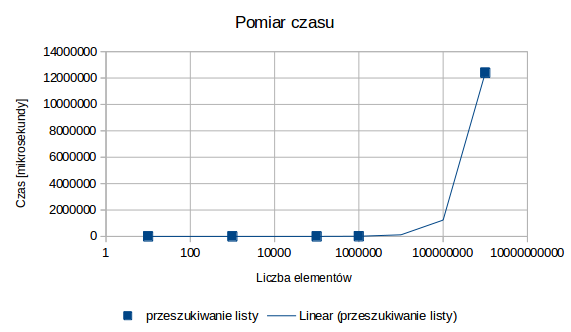
\includegraphics[scale=0.6]{../wyniki/wyniki_przeszukania.png}
\end{center}
\caption{Zobrazowanie wyników pomiaru oraz regresja liniowa wykonana w programie \textit{LibreOffice Calc}.}
\end{figure}

\begin{table}[htbp]
\begin{center}
\begin{tabular}{|c|>{\centering\arraybackslash}p{1,5cm}|>{\centering\arraybackslash}p{1,5cm}|>{\centering\arraybackslash}p{1,5cm}|>{\centering\arraybackslash}p{1,5cm}|>{\centering\arraybackslash}p{1,5cm}|}
\hline
\multicolumn{1}{|l|}{} & \multicolumn{ 5}{c|}{\textbf{Pomiary czasu przeszukiwania listy n-elementowej}} \\ \hline
\textbf{Ilość elementów} & $10$ & $10^3$& $10^5$ & $10^6$ & $10^9$ \\ \hline
\textbf{Pomiar 1 [us]} & 27 & 14 & 801 & 10848 & 5118450 \\ \hline
\textbf{Pomiar 2 [us]} & 12 & 14 & 731 & 10299 & 5157010 \\ \hline
\textbf{Pomiar 3 [us]} & 8 & 13 & 727 & 10598 & 5119420 \\ \hline
\textbf{Pomiar 4 [us]} & 7 & 15 & 654 & 11445 & 5010000 \\ \hline
\textbf{Pomiar 5 [us]} & 6 & 15 & 598 & 10950 & 4807910 \\ \hline
\textbf{Pomiar 6 [us]} & 7 & 15 & 618 & 10011 & 4667350 \\ \hline
\textbf{Pomiar 7 [us]} & 8 & 14 & 858 & 10036 & 4824640 \\ \hline
\textbf{Pomiar 8 [us]} & 6 & 15 & 880 & 11255 & 4808720 \\ \hline
\textbf{Pomiar 9 [us]} & 8 & 14 & 856 & 10754 & 5056860 \\ \hline
\textbf{Pomiar 10 [us]} & 6 & 15 & 842 & 10385 & 5362980 \\ \hline
\textbf{Pomiar 11 [us]} & 6 & 15 & 925 & 11173 & 5631260 \\ \hline
\textbf{Pomiar 12 [us]} & 6 & 15 & 860 & 12431 & 4804130 \\ \hline
\textbf{Pomiar 13 [us]} & 8 & 15 & 875 & 10471 & 5053090 \\ \hline
\textbf{Pomiar 14 [us]} & 7 & 14 & 860 & 11501 & 5456830 \\ \hline
\textbf{Pomiar 15 [us]} & 6 & 15 & 635 & 10718 & 5152060 \\ \hline
\textbf{Pomiar 16 [us]} & 8 & 14 & 568 & 10621 & 4728930 \\ \hline
\textbf{Pomiar 17 [us]} & 6 & 14 & 566 & 10085 & 4709380 \\ \hline
\textbf{Pomiar 18 [us]} & 7 & 15 & 576 & 10755 & 4858750 \\ \hline
\textbf{Pomiar 19 [us]} & 7 & 15 & 566 & 10625 & 4746280 \\ \hline
\textbf{Pomiar 20 [us]} & 6 & 15 & 566 & 10638 & 5122880 \\ \hline
\textbf{Pomiar 21 [us]} & 7 & 14 & 768 & 10338 & 5021030 \\ \hline
\textbf{Pomiar 22 [us]} & 7 & 14 & 776 & 10423 & 5198310 \\ \hline
\textbf{Pomiar 23 [us]} & 7 & 15 & 803 & 10671 & 4938670 \\ \hline
\textbf{Pomiar 24 [us]} & 6 & 15 & 568 & 10110 & 5447080 \\ \hline
\textbf{Pomiar 25 [us]} & 7 & 14 & 557 & 9994 & 4762510 \\ \hline
\textbf{Pomiar 26 [us]} & 8 & 14 & 567 & 10343 & 4828810 \\ \hline
\textbf{Pomiar 27 [us]} & 6 & 15 & 598 & 10312 & 5148940 \\ \hline
\textbf{Pomiar 28 [us]} & 6 & 15 & 589 & 10330 & 5413450 \\ \hline
\textbf{Pomiar 29 [us]} & 7 & 13 & 598 & 10281 & 6023600 \\ \hline
\textbf{Pomiar 30 [us]} & 7 & 14 & 583 & 10351 & 5554910 \\ \hline
\textbf{Pomiar 31 [us]} & 7 & 13 & 579 & 10339 & 4938560 \\ \hline
\textbf{Pomiar 32 [us]} & 7 & 13 & 550 & 10541 & 5009070 \\ \hline
\textbf{Pomiar 33 [us]} & 6 & 13 & 556 & 10269 & 4969610 \\ \hline
\textbf{Pomiar 34 [us]} & 8 & 13 & 557 & 9980 & 5448210 \\ \hline
\textbf{Pomiar 35 [us]} & 7 & 14 & 731 & 10766 & 5188510 \\ \hline
\textbf{Pomiar 36 [us]} & 6 & 13 & 851 & 10066 & 5341730 \\ \hline
\textbf{Pomiar 37 [us]} & 8 & 13 & 769 & 10103 & 4893010 \\ \hline
\textbf{Pomiar 38 [us]} & 7 & 14 & 577 & 10728 & 4950110 \\ \hline
\textbf{Pomiar 39 [us]} & 7 & 14 & 565 & 9956 & 5033890 \\ \hline
\textbf{Pomiar 40 [us]} & 8 & 13 & 558 & 10198 & 5106000 \\ \hline
\textbf{Pomiar 41 [us]} & 7 & 14 & 557 & 10881 & 4836780 \\ \hline
\textbf{Pomiar 42 [us]} & 8 & 14 & 721 & 9890 & 4740970 \\ \hline
\textbf{Pomiar 43 [us]} & 6 & 13 & 827 & 9964 & 4676980 \\ \hline
\textbf{Pomiar 44 [us]} & 7 & 14 & 568 & 10792 & 4591480 \\ \hline
\textbf{Pomiar 45 [us]} & 7 & 13 & 551 & 9892 & 4593950 \\ \hline
\textbf{Pomiar 46 [us]} & 7 & 13 & 653 & 12217 & 4604570 \\ \hline
\textbf{Pomiar 47 [us]} & 7 & 14 & 562 & 11086 & 4696340 \\ \hline
\textbf{Pomiar 48 [us]} & 7 & 21 & 615 & 10414 & 4782500 \\ \hline
\textbf{Pomiar 49 [us]} & 8 & 13 & 612 & 11306 & 4792440 \\ \hline
\textbf{Pomiar 50 [us]} & 7 & 13 & 551 & 10386 & 4709200 \\ \hline
\end{tabular}
\end{center}
\label{wyniki1}
\end{table}

\newpage

\begin{table}[htbp]
\caption{}
\begin{center}
\begin{tabular}{|c|c|c|c|c|c|}
\hline
\multicolumn{1}{|l|}{} & \multicolumn{ 5}{c|}{\textbf{Uśredniony czas przeszukiwania listy}} \\ \hline
\textbf{Ilość elementów} & $10$ & $10^3$& $10^5$ & $10^6$ & $10^9$ \\ \hline
\textbf{Szukany indeks} & 5 & 180 & 47 180 & 847 180 & 403 878 424 \\ \hline
\textbf{Szukany indeks (procentowo)} & 50,00\% & 18,00\% & 47,18\% & 84,72\% & 40,39\% \\ \hline
\textbf{Średnia [us]} & 7,44 & 14,18 & 669,58 & 10 570,52 & 5 008 763 \\ \hline
\end{tabular}
\end{center}
\label{wyniki2}
\end{table}



\begin{table}[htbp]
\caption{}
\begin{center}
\begin{tabular}{|c|c|c|c|c|c|}
\hline
\multicolumn{1}{|l|}{} & \multicolumn{ 5}{c|}{\textbf{Predykcja – ile zajęłoby czasu przeszukanie całej listy}} \\ \hline
\textbf{Ilość elementów} & $10$ & $10^3$& $10^5$ & $10^6$ & $10^9$ \\ \hline
\textbf{Średnia [us]} & 14,88 & 78,78& 1 419,21& 12 477,31& 12 401 660,26\\ \hline
\end{tabular}
\end{center}
\label{wyniki3}
\end{table}

\bigskip

Po ostatniej tabeli wyraźnie widać, że wyszukiwanie elementów do tablicy ma złożoność obliczeniową rowną O(n). Najlepiej można to zaobserwować porównując predykcję dla miliona i miliarda elementów. Dzięki dużej ilości danych, bardzo zmalał błąd pomiaru czasu i można zaobserwować proporcjonalny wzrost czasu wyszukiwania - 1000 razy większy dla 1000 razy większej próbki.

\section{Wnioski}
\hspace{4ex}Dysponując podanymi danymi oraz stojącą za nimi teorią zakwalifikowałbym przeszukanie tablicy jako algorytm rzędu O($n$). Podczas implementacji algorytmu dowiedziałem się dlaczego implementacja tablicowa jest dużo lepsza. Pozwala na szybszy zapis ze względu na to, że alokacja pamięci następuje w złożoności obliczeniowej O($nlog(n)$) a nie O($n^2$).
\end{document}